\sloppy
\documentclass[14pt,a4paper,oneside]{extarticle}	% Размер основного шрифта и формата листа
\usepackage{xltxtra}						% Используется для вывода логотипа XeLaTeX
\usepackage{xunicode}						% Кодировка документа
\usepackage{polyglossia}					% Загружает пакет многоязыковой верстки
\newfontfamily\russianfont{Book Antiqua}
%\setmainfont{Liberation Serif}						% Основной шрифт текста
\setmainfont{Book Antiqua}
\setdefaultlanguage{russian}				% Основной язык текста
\setotherlanguage{english}					% Дополнительный язык текста
\linespread{1}							% Межстрочный интервал выбран полуторным
\usepackage[left=2.5cm,
right=1.5cm,vmargin=2.5cm]{geometry} % Отступы по краям листа
\bibliographystyle{ugost2008}

\usepackage{xcolor}
\usepackage{hyperref}
% Цвета для гиперссылок
\definecolor{linkcolor}{HTML}{359B08} % цвет ссылок
\definecolor{urlcolor}{HTML}{799B03} % цвет гиперссылок
\hypersetup{pdfstartview=FitH,  linkcolor=linkcolor,urlcolor=urlcolor, colorlinks=true}

%---------------------------%
%---- Пакеты расширений ----%
%---------------------------%
\usepackage{xcolor}
\usepackage{hyperref}
% Цвета для гиперссылок
\definecolor{linkcolor}{HTML}{359B08} % цвет ссылок
\definecolor{urlcolor}{HTML}{799B03} % цвет гиперссылок
\hypersetup{pdfstartview=FitH,  linkcolor=linkcolor,urlcolor=urlcolor, colorlinks=true}


\usepackage{verbatim,indentfirst}
\usepackage{cite,enumerate,float}
\usepackage{amsmath,amssymb,amsthm,amsfonts}

%---------------------------%
%--- Вставка иллюстраций ---%
%---------------------------%
\usepackage{graphicx}
\usepackage{subfigure}
%\graphicspath{{Images/}}
\usepackage{fontspec}

\begin{document}
%	\pagestyle{empty} %  выключаенм нумерацию

	%\setcounter{page}{3}% Нумерация начинается с третьей страницы
	%\renewcommand{\contentsname}{\center{Содержание}}
	%\tableofcontents
	
	\begin{center}
		%\addcontentsline{toc}{section}{Опыт 13. Сухое трение. Трибометр Кулона}
		\subsection*{Силы сухого трения}
	\end{center}
	
	\begin{figure}[H]
		\centering 	
		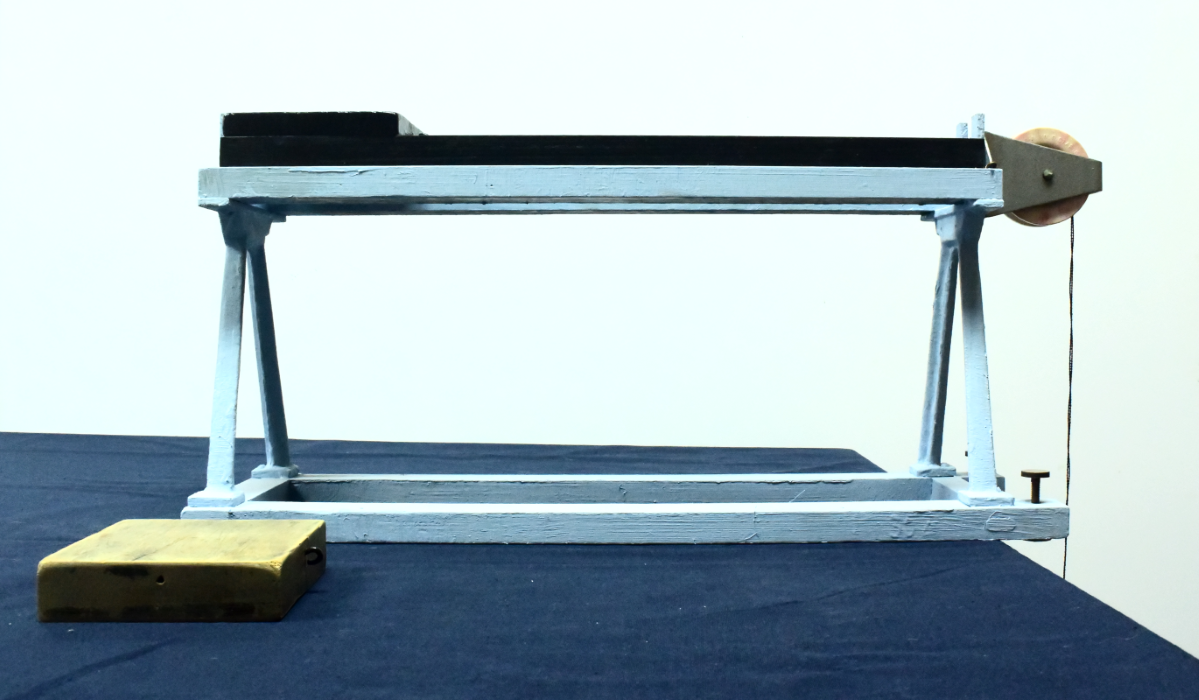
\includegraphics[width=0.9\linewidth]{friction-4.png}
		\caption{Демонстрация трения покоя и трения скольжения}
		\label{friction-4}
	\end{figure}
	
	\subsection*{\underline{Оборудование:}}
	
	\begin{enumerate} 
		\item Трибометр Кулона
		\item Разновесы массой 100 г каждый
		\item Бруски из сосны и железа
		
	\end{enumerate}

	\newpage	
	\subsection*{\underline{Основные определения:}}
	
Силы трения могут возникать при непосредственном соприкосновении твердых тел.
Для этих сил характерно то, что они действуют вдоль поверхности соприкосновения и всегда направлены 
	так, что препятствуют движению соприкасающихся тел друг относительно друга.
	Эти силы часто называют силами сухого трения. 
	Здесь будет рассмотрено только два вида сил сухого трения: трение покоя 
	и трение скольжения (трение качения опускается).
	
	Трение — диссипативный процесс, 
	сопровождающийся выделением тепла, электризацией тел, их разрушением и т. д. 
	Характеристикой трения скольжения выступает коэффициент трения 
	скольжения — безразмерная величина, равная отношению силы трения к нормальной нагрузке.
	Внешние условия (нагрузка, скорость, 
	 шероховатость, температура, смазка) влияют на величину 
	 трения не меньше, чем природа трущихся тел, меняя его в несколько раз.
	
	Если начать действовать с малой силой \textbf{F}, то предмет не сдвинется с места. 
	Он останется в покое потому, что одновременно с силой \textbf{F} на него начнет действовать со 
	стороны пола сила трения покоя $ \textbf{F}_{\text{тp}} $.
	Эта сила $ \textbf{F}_{\text{тp}} $ по модулю равна внешней силе \textbf{F}, но направлена в противоположную сторону и препятствует 	возникновению движения.
	Одновременно с изменениями модуля и направления внешней силы сила трения покоя тоже меняет свой 
	модуль и направление. 	
	
	Трибометрия — методы измерения силы или 
	коэффициента трения, порога трения и величины износа трущихся поверхностей. 
	Трибометрические измерения делятся на два вида: 
	лабораторные, при которых производится оценка сил трения и износостойкости материалов 
	в тех или иных условиях, и натурные, когда производится оценка целиком данного узла трения.

	\newpage	
	\subsection*{\underline{Краткое описание:}}
	
	Прибор состоит из плоскости, образуемой отполированными металлическими направляющими, и угол наклона этой плоскости можно менять.
	В ходе опытов используется железный и деревянный брусок, широкие грани которых имеют одинаковую площадь.
	Прибор можно использовать для демонстраций многих эффектов, связанных с трением.
	
	\textit{Наклонный трибометр}.	
	Поместив стальной брусок на трибометр гладкой стороной, необходимо постепенно увеличивать угол наклона плоскости.
	При угле наклона, тангенс которого равен коэффициенту трения, брусок начнет скользить по плоскости.
	Условие для угла наклона плоскости, при котором тело начинает движение, имеет простой вид
		 $$ \text{tg}\alpha=\mu. $$
	Если выполнить опыт с тем же бруском, но расположив его на трибометре шероховатой стороной, 
	то можно заметить, что скольжение начинается при гораздо большем угле наклона плоскости, 
	так как коэффициент трения $  \mu $ в этом случае значительно возрастает.
	
	После этого опыт повторяется с бруском из дерева.
	В ходе демонстрации можно показать, что коэффициент трения не зависит от массы тела.
	Для этого необходимо провести измерения угла с парой деревянных брусков.
	
	\textit{Трение покоя}.	
    В ходе опыта можно определить наибольшее значение силы трения покоя.
    Для этого трибометр необходимо расположить горизонтально на краю стола.
    Брусок помещается на направляющие трибометра, а при помощи нити, перекинутой через шкив, к телу подвешивается груз \textit{m}.
	Если постепенно увеличивать массу груза \textit{m}, то при некоторой нагрузке возникнет скольжение бруска \textit{М} вдоль рельсов. 
	При этом сила трения покоя примет наибольшее возможное значение и станет равна 
	силе тяжести груза \textit{m\textbf{g}}.
	Для проверки брусок и полученный набор разновесов можно взвесить.
	
	Ряд таких простых опытов позволяет установить все основные 
	свойства сил трения скольжения. 
	Опыты показывают, что сила трения скольжения оказывается немного меньше, чем наибольшая 
	сила трения покоя. 

	\newpage	
	\subsection*{\underline{Теория:}}
	
	Используя трибометр, можно подметить важную особенность сил трения покоя: сила трения покоя \textit{\textbf{f}} растет пропорционально силе нормального давления (реакции опоры)
	\textit{\textbf{N}}, прижимающей тела друг к другу. 
	Действительно, нагружая брусок \textit{m} дополнительным грузом, можно увеличивать 
	силу давления и наблюдать повышение наибольшей силы трения, пропорциональное изменению \textit{\textbf{N}}. 
	Поэтому можно записать: 
	\begin{equation}\label{friction-4eq1}
	f_0  = \mu N.
	\end{equation}
	Здесь \textit{N} — сила реакции опоры; постоянная $ \mu $ — коэффициент трения.
	Часто при решении задач, если это не оговаривается дополнительно, используется уравнение $ f_0 = \mu N $ как дополнительное, выражающее особые свойства сил трения скольжения. 

\textit{Брусок на горизонтальной поверхности}.
Рассмотрим вначале брусок массой \textit{m}, расположенный на горизонтальной шероховатой поверхности (рис.\ref{friction-5},\textit{а}).
К телу со стороны одной из боковых граней прикреплена нерастяжимая нить, а на противоположном конце нити находится другой груз, массу \textit{M} которого можно легко менять (разновесы).
Нить перекинута через шкив, поэтому брусок способен перемещаться под действием создаваемой разновесами силы натяжения нити.

Второй закон Ньютона для бруска \textit{m} в векторной форме имеет вид:
\begin{equation}\label{friction-4eq2}
m\textbf{a} = m\textbf{g} + \textbf{N} + \textbf{T} + \textbf{\textit{f}}_0.
\end{equation}
Вдоль оси \textit{y} брусок не совершает движения, значит $ a_y=0 $.
Проектируя уравнение движения на ось \textit{y}, получим равенство: $$ 0 = -mg+N, $$ откуда $$ N=mg. $$
В проекции на ось \textit{x}: $$ 0 = T - f .$$

Максимальная величина силы трения покоя (она же сила трения скольжения)
$ f_0  = \mu N	= \mu mg$.
Следовательно, при условии $ T < \mu mg $ брусок останется на месте и сила трения будет силой трения покоя: $ f = T $.
Если  $ T \geq \mu mg $ (больше максимальной силы трения покоя), то брусок начнет скользить, и сила трения будет силой трения скольжения: $ f =  f_0 = \mu mg $.

\begin{figure}[H] 
	\centering 	
	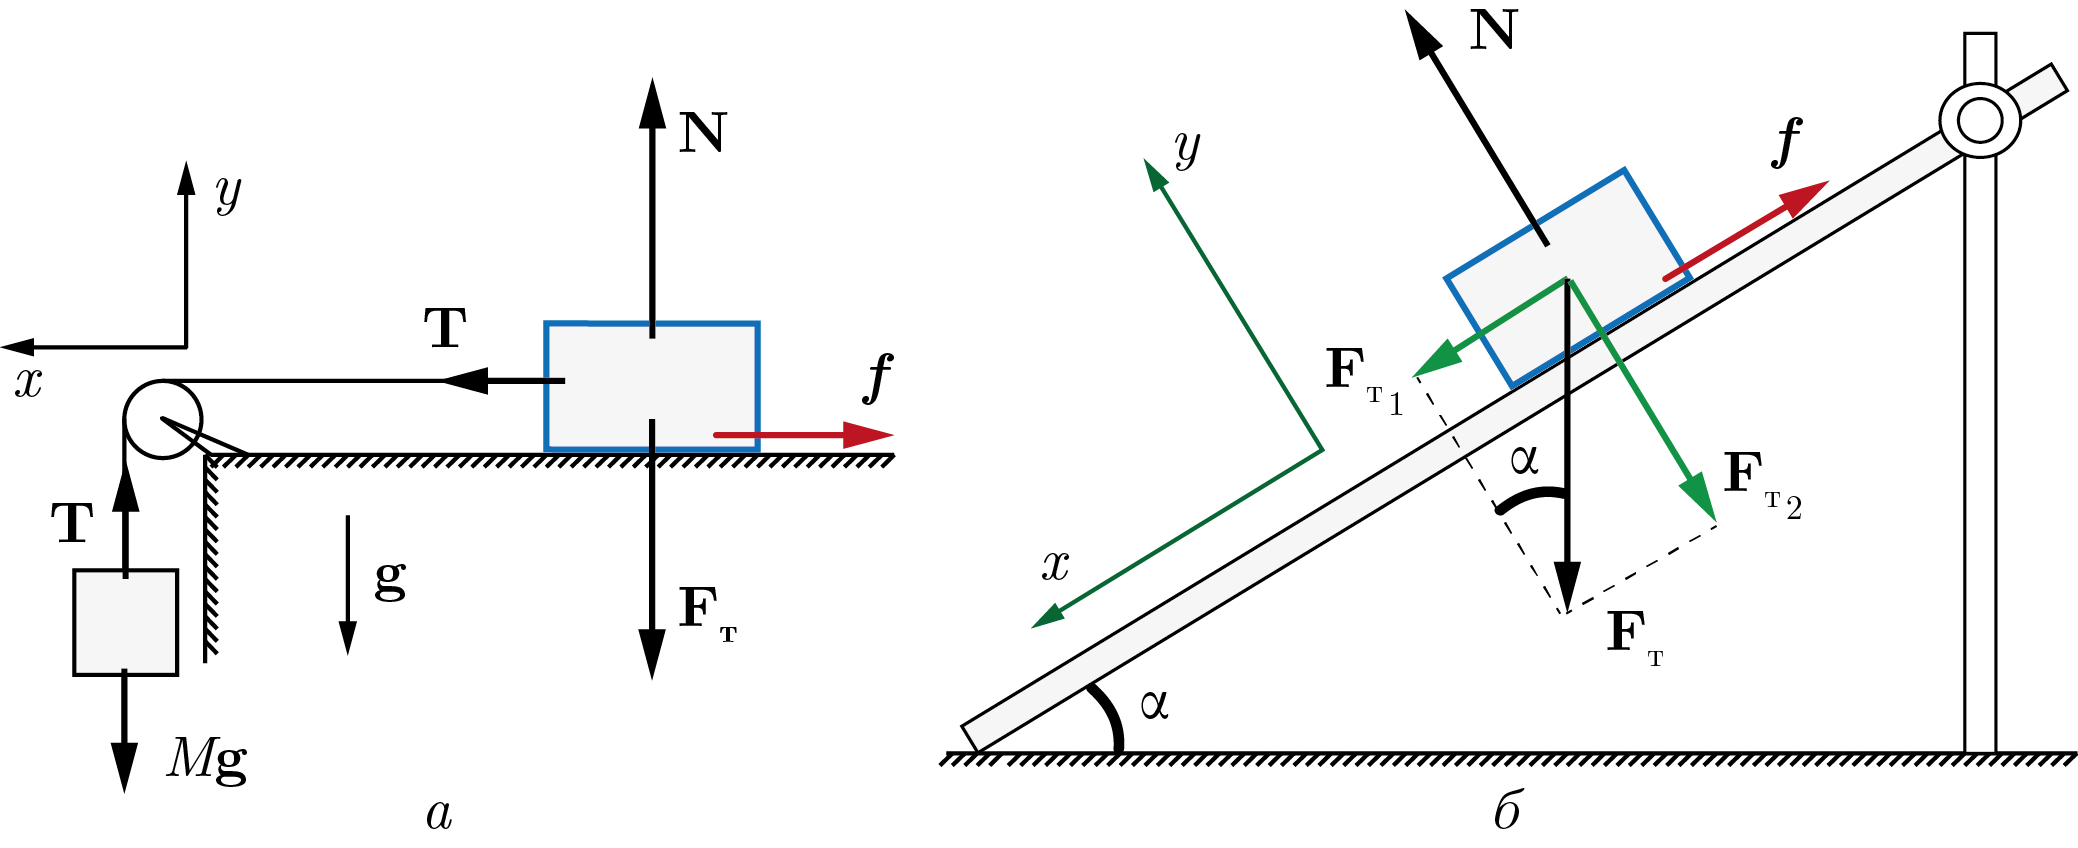
\includegraphics[width=0.9\linewidth]{friction-5.png}
	\caption{\textit{а} — схематичное изображение тела на горизонтальной поверхности и действующие на него силы; \textit{б} — распределение сил, действующих на груз, скатывающийся вдоль наклонной плоскости}
	\label{friction-5}
\end{figure}

\textit{Брусок на наклонной плоскости}.
	
	Для того, чтобы брусок начал движение по наклонной плоскости, ему нужно преодолеть силу трения покоя меньше, чем в случае с горизонтальной плоскостью.
	Движение бруска начинается тогда, когда составляющая $ F_{\text{т}_1} $ силы тяжести, которая действует параллельно плоскости, достигнет величины силы трения покоя $ f_0 $.
Векторная разность между силой тяжести и составляющей $ F_{\text{т}_1} $, направленной вниз по плоскости, выражается составляющей, перпендикулярной плоскости, $ F_{\text{т}_2} $ (рис.\ref{friction-5},\textit{б}).
Величины этих сил определяются проекциями силы тяжести на оси \textit{x} и \textit{y} соответственно:
	\begin{equation}\label{friction-4eq3}
F_{\text{т}_1} = F_{\text{т}}\cdot \text{sin}\alpha, \\F_{\text{т}_2} = F_{\text{т}}\cdot \text{cos}\alpha.
\end{equation}



Ввиду того, что движение бруска происходит при условии $  F_{\text{т}_1}=f_0 $, причем в это же время выполняется равенство $ F_{\text{т}_2}=N $, то связь силы реакции опоры с силой трения скольжения $ f_0 = \mu N $ можно переписать в следующем виде:
	\begin{equation}\label{friction-4eq4}
F_{\text{т}_1} = NF_{\text{т}_2}.
\end{equation}
Тогда
 	\begin{equation}\label{friction-4eq5}
  mg \cdot \text{sin}\alpha = \mu mg \cdot \text{cos}\alpha,
 \end{equation}
откуда следует, что:
 	\begin{equation}\label{friction-4eq6}
\text{tg}\alpha = \mu.
\end{equation}

Тот факт, что составляющая $ F_{\text{т}_1} = mg \cdot\text{sin}\alpha $ меньше полной силы тяжести \textit{mg} ($\text{sin}\alpha < 1$), становится более очевидным по мере уменьшения угла наклона плоскости $ \alpha $.

\end{document}